\documentclass[11pt,letterpaper]{article}
\usepackage[utf8]{inputenc}
\usepackage[left=1in,right=1in,top=1in,bottom=1in]{geometry}
\usepackage{amsfonts,amsmath}
\usepackage{graphicx,float}
% -----------------------------------
\usepackage{hyperref}
\hypersetup{%
  colorlinks=true,
  linkcolor=blue,
  citecolor=blue,
  urlcolor=blue,
  linkbordercolor={0 0 1}
}
% -----------------------------------
\usepackage[style=authoryear-icomp,backend=biber]{biblatex}
\addbibresource{citation.bib}
% -----------------------------------
\usepackage{fancyhdr}
\newcommand\course{MATH-UA.0252\\Numerical Analysis}
\newcommand\hwnumber{8}                  % <-- homework number
\newcommand\NetIDa{Ryan Sh\`iji\'e D\`u} 
\newcommand\NetIDb{November 3rd, 2023}
\pagestyle{fancyplain}
\headheight 35pt
\lhead{\NetIDa\\\NetIDb}
\chead{\textbf{\Large Worksheet \hwnumber}}
\rhead{\course}
\lfoot{}
\cfoot{}
\rfoot{\small\thepage}
\headsep 1.5em
% -----------------------------------
\usepackage{titlesec}
\renewcommand\thesubsection{(\arabic{section}.\alph{subsection})}
\titleformat{\subsection}[runin]
        {\normalfont\bfseries}
        {\thesubsection}% the label and number
        {0.5em}% space between label/number and subsection title
        {}% formatting commands applied just to subsection title
        []% punctuation or other commands following subsection title
% -----------------------------------
\setlength{\parindent}{0.0in}
\setlength{\parskip}{0.1in}
% -----------------------------------
\newcommand{\de}{\mathrm{d}}
\newcommand{\DD}{\mathrm{D}}
\newcommand{\pe}{\partial}
\newcommand{\mcal}{\mathcal}
%\newcommand{\pdx}{\left|\frac{\partial}{\partial_x}\right|}

\newcommand{\dsp}{\displaystyle}

\newcommand{\norm}[1]{\left\Vert #1 \right\Vert}
%\newcommand{\mean}[1]{\left\langle #1 \right\rangle}
\newcommand{\mean}[1]{\overline{#1}}
\newcommand{\inner}[2]{\left\langle #1,#2\right\rangle}

\newcommand{\ve}[1]{\boldsymbol{#1}}

\newcommand{\thus}{\Rightarrow \quad }
\newcommand{\fff}{\iff\quad}
\newcommand{\qdt}[1]{\quad \mbox{#1} \quad}

\renewcommand{\Re}{\mathrm{Re}}
\renewcommand{\Im}{\mathrm{Im}}
\newcommand{\E}{\mathbb{E}}
\newcommand{\lap} {\nabla^2}
\renewcommand{\div}{\nabla\cdot}

\newcommand{\csch}{\text{csch}}
\newcommand{\sech}{\text{sech}}


\newcommand{\hot}{\text{h.o.t.}}

\newcommand{\ssp}{\left.\qquad\right.}

\newcommand{\var}{\text{var}}
\newcommand{\cov}{\text{cov}}

%%%%%%%%%%%%%%%%%%%%%%%%%%%%%%%%%%%%%%%%%%%%%%%%%%
\makeatletter
\newcommand*{\mint}[1]{%
  % #1: overlay symbol
  \mint@l{#1}{}%
}
\newcommand*{\mint@l}[2]{%
  % #1: overlay symbol
  % #2: limits
  \@ifnextchar\limits{%
    \mint@l{#1}%
  }{%
    \@ifnextchar\nolimits{%
      \mint@l{#1}%
    }{%
      \@ifnextchar\displaylimits{%
        \mint@l{#1}%
      }{%
        \mint@s{#2}{#1}%
      }%
    }%
  }%
}
\newcommand*{\mint@s}[2]{%
  % #1: limits
  % #2: overlay symbol
  \@ifnextchar_{%
    \mint@sub{#1}{#2}%
  }{%
    \@ifnextchar^{%
      \mint@sup{#1}{#2}%
    }{%
      \mint@{#1}{#2}{}{}%
    }%
  }%
}
\def\mint@sub#1#2_#3{%
  \@ifnextchar^{%
    \mint@sub@sup{#1}{#2}{#3}%
  }{%
    \mint@{#1}{#2}{#3}{}%
  }%
}
\def\mint@sup#1#2^#3{%
  \@ifnextchar_{%
    \mint@sup@sub{#1}{#2}{#3}%
  }{%
    \mint@{#1}{#2}{}{#3}%
  }%
}
\def\mint@sub@sup#1#2#3^#4{%
  \mint@{#1}{#2}{#3}{#4}%
}
\def\mint@sup@sub#1#2#3_#4{%
  \mint@{#1}{#2}{#4}{#3}%
}
\newcommand*{\mint@}[4]{%
  % #1: \limits, \nolimits, \displaylimits
  % #2: overlay symbol: -, =, ...
  % #3: subscript
  % #4: superscript
  \mathop{}%
  \mkern-\thinmuskip
  \mathchoice{%
    \mint@@{#1}{#2}{#3}{#4}%
        \displaystyle\textstyle\scriptstyle
  }{%
    \mint@@{#1}{#2}{#3}{#4}%
        \textstyle\scriptstyle\scriptstyle
  }{%
    \mint@@{#1}{#2}{#3}{#4}%
        \scriptstyle\scriptscriptstyle\scriptscriptstyle
  }{%
    \mint@@{#1}{#2}{#3}{#4}%
        \scriptscriptstyle\scriptscriptstyle\scriptscriptstyle
  }%
  \mkern-\thinmuskip
  \int#1%
  \ifx\\#3\\\else_{#3}\fi
  \ifx\\#4\\\else^{#4}\fi  
}
\newcommand*{\mint@@}[7]{%
  % #1: limits
  % #2: overlay symbol
  % #3: subscript
  % #4: superscript
  % #5: math style
  % #6: math style for overlay symbol
  % #7: math style for subscript/superscript
  \begingroup
    \sbox0{$#5\int\m@th$}%
    \sbox2{$#5\int_{}\m@th$}%
    \dimen2=\wd0 %
    % => \dimen2 = width of \int
    \let\mint@limits=#1\relax
    \ifx\mint@limits\relax
      \sbox4{$#5\int_{\kern1sp}^{\kern1sp}\m@th$}%
      \ifdim\wd4>\wd2 %
        \let\mint@limits=\nolimits
      \else
        \let\mint@limits=\limits
      \fi
    \fi
    \ifx\mint@limits\displaylimits
      \ifx#5\displaystyle
        \let\mint@limits=\limits
      \fi
    \fi
    \ifx\mint@limits\limits
      \sbox0{$#7#3\m@th$}%
      \sbox2{$#7#4\m@th$}%
      \ifdim\wd0>\dimen2 %
        \dimen2=\wd0 %
      \fi
      \ifdim\wd2>\dimen2 %
        \dimen2=\wd2 %
      \fi
    \fi
    \rlap{%
      $#5%
        \vcenter{%
          \hbox to\dimen2{%
            \hss
            $#6{#2}\m@th$%
            \hss
          }%
        }%
      $%
    }%
  \endgroup
}

\begin{document} 

\section{Computing eigenvalues via the Power Iteration}
Given is the following matrix:
\[
A=\begin{bmatrix}
-2 & 1 & 4  \\ 1 & 1 & 1 \\ 4 & 1 & -2 \end{bmatrix},
\]
It has eigenvalues and eigenvectors:
\[
\lambda_1=0,
\, {\boldsymbol v_1}
=\begin{bmatrix}
0.41  \\ -0.82 \\ 0.41 \end{bmatrix},\quad
\lambda_2=-6,
\,{\boldsymbol v_2}
=\begin{bmatrix}
0.71  \\ 0.0 \\ -0.71 \end{bmatrix},\quad
\lambda_3=3, \,{\boldsymbol v_3}
=\begin{bmatrix}
-0.58  \\ -0.58 \\ -0.58 \end{bmatrix}.
\]

\subsection{}\label{sec:1.a}
Calculate the first iterate of the power method when ${\boldsymbol x_0}=(0,1,1)^T$.

\subsection{}
Which eigenvalue direction will the sequence defined in \ref{sec:1.a} converge to?
  
\subsection{}
Give an initialization vector such that the power method does \emph{not} converge to the direction of the largest (in absolute value) eigenvalue.
  
\subsection{}\label{sec:1d}
Write a simple program implementing the power method for the matrix $A$.
\begin{enumerate}
    \item Use the Rayleigh quotient to calculate estimates of the eigenvalues for each iteration.
    \item What is the order of convergence of the eigenvector estimates and the eigenvalue estimates? What is the speed of convergence?
    \item Could you explain the relationship between the two convergence speeds? \\
    (Hint: last week we showed that eigenvectors $\ve v$ are stationary points of the Rayleigh quotient)
\end{enumerate}

\section{The Inverse Iteration}
Take $A$ to be the matrix above, and let $\theta\in\mathbb{R}$ and let ${\boldsymbol x_0}\in\mathbb{R}^3$.
\subsection{}
Define the \emph{Inverse Iteration} (also called
  \emph{Inverse Power Method}) to calculate eigenvectors of $A$ near
  $\theta$.

\subsection{}
If $\theta=2$, where will the sequence defined in (i)
  converge to and why?

\subsection{}
If $\theta=-2$, where will the sequence defined in (i)
  converge to and why?

\subsection{}
Write a simple program implementing the inverse power method. Do the same sub-tasks as the ones in \ref{sec:1d}.

\section{The Rayleigh Quotient Iteration}
It is irresistible to use the eigenvalues estimates from the Rayleigh quotient to update $\theta$ for each step in the inverse iteration. The resulting algorithm is the Rayleigh Quotient Iteration \parencite{TrefethenBau_97}:
\begin{figure}[H]
    \centering
    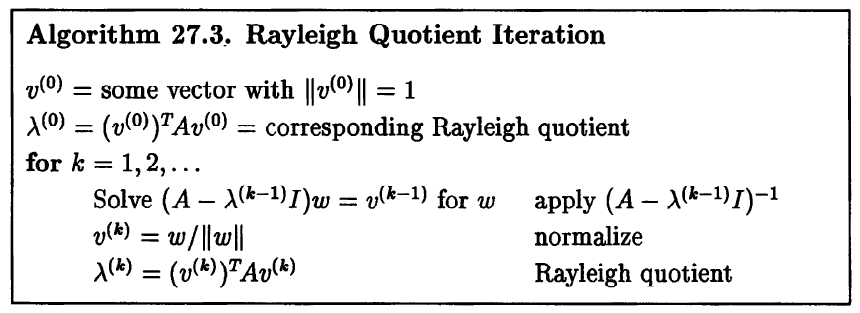
\includegraphics[width = 0.8\textwidth]{Session_8/latex/figs/TB_Rayleigh_Quo_Iter}
\end{figure}

\subsection{}
Implement the Rayleigh Quotient Iteration. 
\begin{enumerate}
    \item What is the order of convergence of the eigenvector estimates and the eigenvalue estimates?
    \item Could you explain this (high) order of convergence?
\end{enumerate}

\vfill
\printbibliography

\end{document}